\section{Lazo de control para regular el filamento}
\label{sec:reg_expt}

Durante las producciones realizadas anteriormente, se ha notado que existe una relación entre la velocidad de tracción y el diámetro final del filamento, sin embargo, el sistema que se dispone carece de la robustez necesaria para poder trabajar con un regulador del tipo PID, en el que es necesario conocer de manera lo más exacta posible, la distribución de la planta con la que se trabaja. Además el número de perturbaciones que afectan a nuestro sistema es demasiado amplio y no se puede llegar a tener control de todas y cada una de ellas.)\\

Como se puede ver en la Figura \ref{fig:reg_mezcla}, la salida de filamento que proporciona el filastruder no es constante y en ocasiones, no está bien mezclada:

\begin{figure}[H]
    \centering
    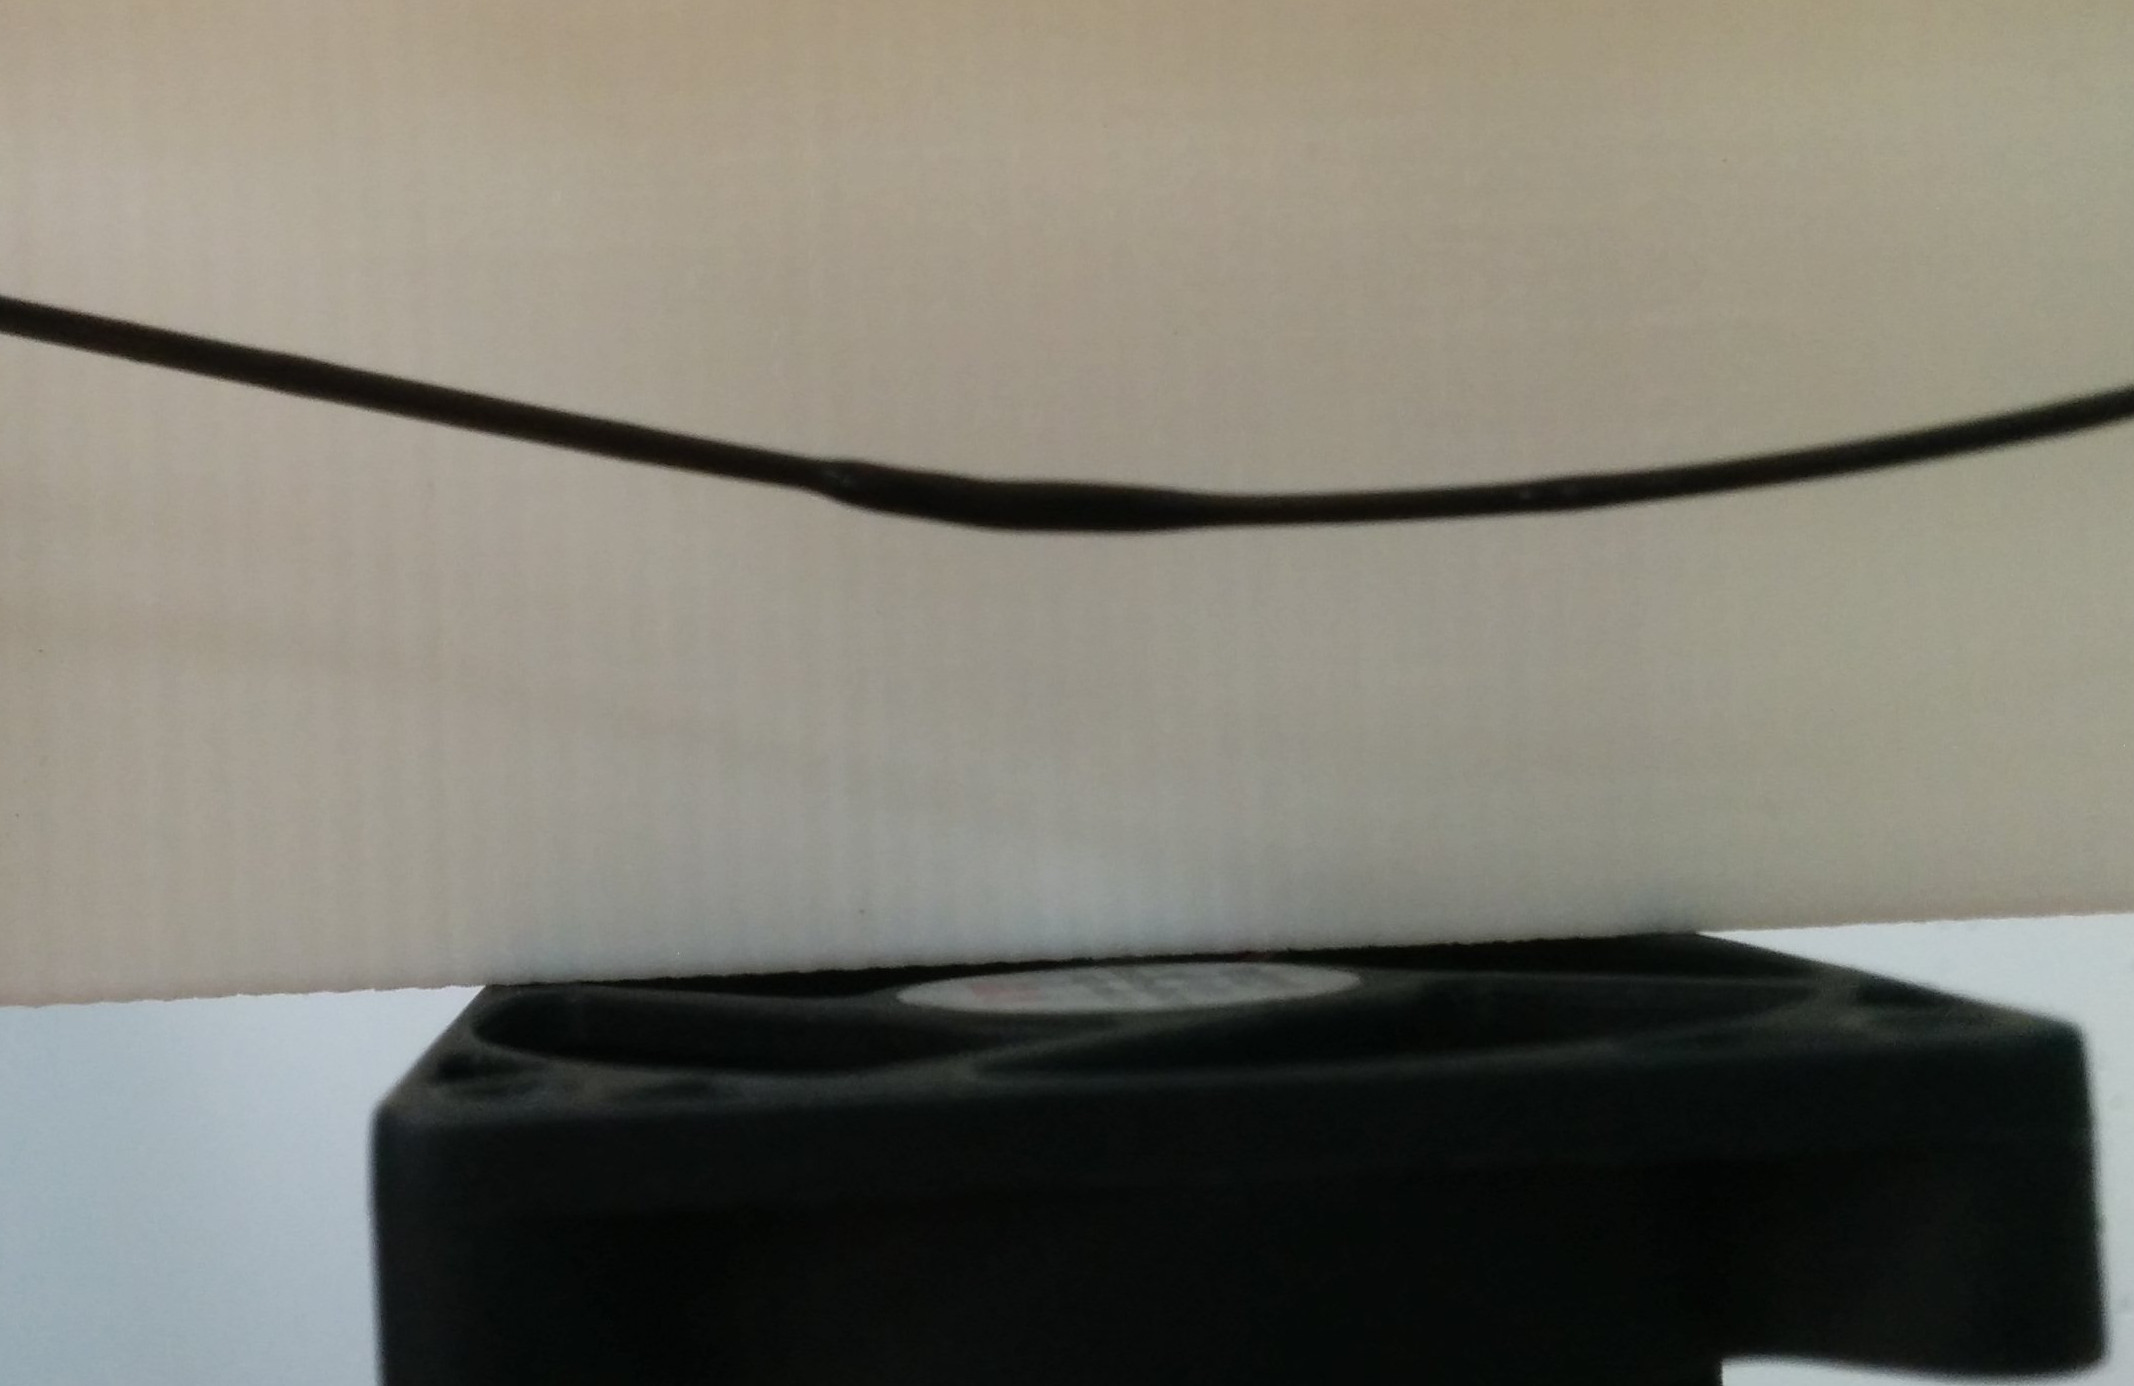
\includegraphics[width=0.6\textwidth]{images/producciones/22072015/IMG_20150722_120959.jpg}
    \caption[Mezcla incorrecta de la filastruder.]{Mezcla incorrecta de la filastruder. Algunos trozos de granza no son mezclados de forma correcta antes de salir del extrusor.}
    \label{fig:reg_mezcla}
\end{figure}

Por ello, se decide no usar un regulador PID e intentar implementar un regulador experto, el cual, imitará las acciones que un humano tomaría para resolver el problema. Este tipo de reguladores se basan en un conocimiento previamente adquirido por una persona, que ha trabajado con el sistema. Para implementear este sistema, se definen una serie de reglas, en las que acotaremos los diámetros del filamento en regiones, y dependiendo, de si el diámetro crece o decrece, se actuará sobre la velocidad de tracción. La Figura \ref{fig:reg_reglas} muestra en más detalle las reglas que se van a utilizar en el regulador.

\begin{figure}[H]
    \centering
    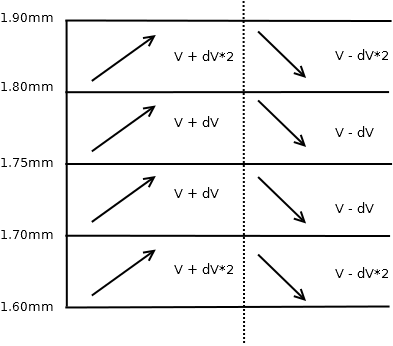
\includegraphics[width=0.5\textwidth]{images/producciones/11082015/Diagram1.png}
    \caption[Reglas a utilizar en el sistema experto.]{Reglas a utilizar en el sistema experto. En función de la zona en la que estemos aplicaremos un incremento positivo o negativo a la velocidad.}
    \label{fig:reg_reglas}
\end{figure}

Separamos en cuatro tramos los diámetros comprendidos entre $1.60mm$ y $1.90mm$, así mismo, también diferenciamos el sentido de avance entre las zonas, tanto si es descendente como descendente. De esta manera podremos tener un control más preciso sobre la velocidad, pudiendo diferenciar tramo y la tendencia que toma el diámetro.

En el Anexo \ref{ane:resultados_regu} se detallan diferentes experimentos que se han realizado modificando estás reglas del regulador, para comprobar su influencia en el diámetro.\\

Tomando los datos obtenidos en el Ensayo 6 \fullref{lab:4} vamos a pasar a compararlos con los datos obtenidos de dos fabricantes distintos de filamento, en la Tabla \ref{tab:compara_results}.

\begin{table}[H]
	\centering
	\begin{tabular}{ccccccc}
		                    & BQ & FormFutura & Filastruder \\ \hline
		Medidas             & 291      &291       & 291      \\
		Media (mm)          & 1.75     & 1.70     & 1.74      \\
		Desviación estandar & 0.01     & 0.05     & 0.21      \\
		min(mm)             & 1.67     & 1.64     & 1.01      \\
		max(mm)             & 1.77     & 1.71     & 2.14     
	\end{tabular}
	\caption{Tabla comparativa de los resultados obtenidos}
	\label{tab:compara_results}
\end{table}

\begin{figure}[H]
    \centering
    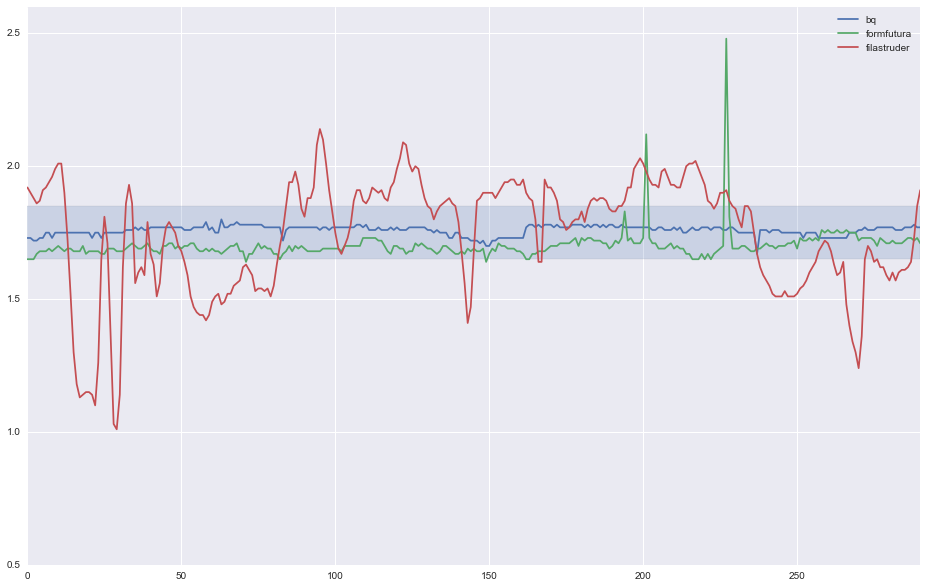
\includegraphics[width=0.99\textwidth]{images/producciones/conclusiones/output_8_1.png}
    \caption{Comparativa filamentos distintos fabricantes}
    \label{fig:concl_graf5}
\end{figure}

\begin{figure}[H]
    \centering
    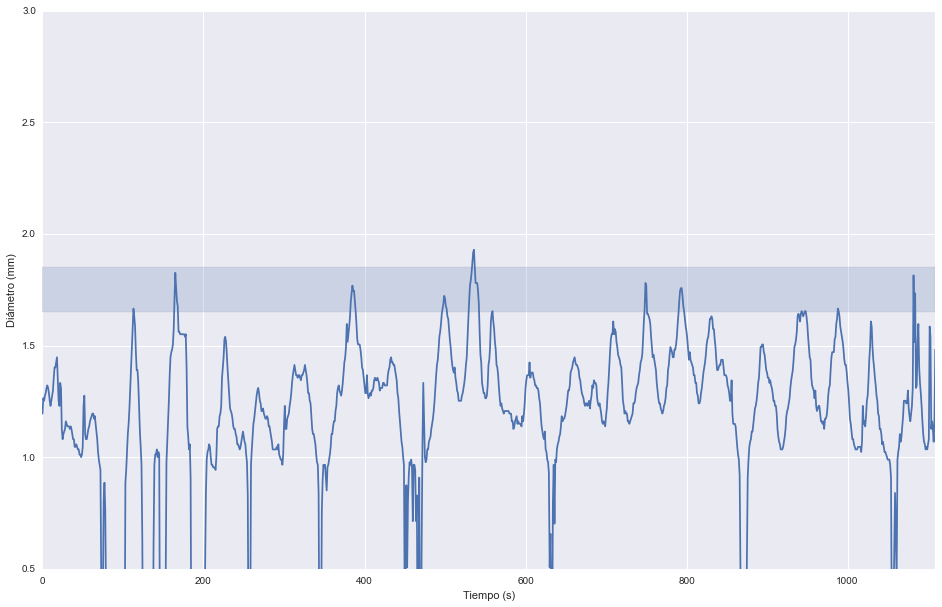
\includegraphics[width=0.6\textwidth]{images/producciones/conclusiones/output_9_1.png}
    \caption{Diagrama de cajas con diámetros de distintos fabricantes}
    \label{fig:concl_cajas5}
\end{figure}

Como podemos observar en los datos, el diámetro de los filamentos que proporcionan empresas como BQ y formfutura, tienen unos valores mucho más estables que los obtenidos con Filastruder. Lo cual es normal debido a la maquinaría y condiciones de trabajo en los que se han realizado en los experimentos. Como se aprecia, el filamento de BQ cumple exactamente las condiciones requeridas en un principo, tener un diámetro nominal  de $1.75mm$ y estar comprendido entre los márgenes de $1.65mm$ y $1.85mm$. Sin embargo, no podemos olvidar que el objetivo principal de nuestro proyecto era crear un sistema de adquisición de datos para gestionar la calidad del filamento, es por eso, que para realizar la comparación se ha escogido una bobina que cumplía los requisitos, pudiendo así comprobar la fiabilidad de nuestro sistema.\\

No obstante, el problema de calidad que se tiene en las bobinas es una realidad, y debido a que no se tiene una completa trazabailidad de los datos de producción, es muy dificil localizar qué bobinas son las que están defectuosas hasta que son usadas en una impresora.

\section{Discusión de los resultados obtenidos}

Tras los distintos experimientos que hemos realizado, podemos concluir que los datos adquiridios por el sistema de adquisición de datos, nos han sido útiles para comprobar cómo funcionaba la extrusora, y en caso de detectar un error, hemos sido capaces de encontrar los motivos ayudándonos del mismo.\\

Uno de los errores detectados ha sido la variación en el flujo másico de salida en el extrusor. Para ello, fuimos capaces de realizar las medidas necesarias para comprobar que había un error y analizando los datos obtenidos, llegar a la conclusión de dónde estaba el problema.\\

A pesar de conocer el error que existía en la extrusora, no se ha decidido invertir tiempo en su reparación debido a que no suponía un impedimento en la realización del objetivo principal del proyecto. De haber sido parte crítica en la consecución del objetivo, hubieramos planteado su solución, incluso hubieramos llegar a pensar en el diseño propio de una extrusora.\\

También hemos podido realizar un pequeño estudio de la influencia de un regulador experto en el diámetro del filamento, no podemos afirmar que el regulador funcioné ya que en las pruebas realizadas la extrusora usada no funcionaba correctamene, pero si podemos afirmar, que los datos obtenidos con nuestro sistema de adquisicón de datos, nos han sido útiles para poder obtener un modelo de nuestro sistema.\\